\documentclass{beamer}
\mode<presentation>
\usepackage{amsmath,amssymb,mathtools}
\usepackage{textcomp}
\usepackage{gensymb}
\usepackage{adjustbox}
\usepackage{subcaption}
\usepackage{enumitem}
\usepackage{multicol}
\usepackage{listings}
\usepackage{url}
\usepackage{graphicx} % <-- needed for images
\def\UrlBreaks{\do\/\do-}

\usetheme{Boadilla}
\usecolortheme{lily}
\setbeamertemplate{footline}{
  \leavevmode%
  \hbox{%
  \begin{beamercolorbox}[wd=\paperwidth,ht=2ex,dp=1ex,right]{author in head/foot}%
    \insertframenumber{} / \inserttotalframenumber\hspace*{2ex}
  \end{beamercolorbox}}%
  \vskip0pt%
}
\setbeamertemplate{navigation symbols}{}

\lstset{
  frame=single,
  breaklines=true,
  columns=fullflexible,
  basicstyle=\ttfamily\tiny   % tiny font so code fits
}

\numberwithin{equation}{section}

% ---- your macros ----
\providecommand{\nCr}[2]{\,^{#1}C_{#2}}
\providecommand{\nPr}[2]{\,^{#1}P_{#2}}
\providecommand{\mbf}{\mathbf}
\providecommand{\pr}[1]{\ensuremath{\Pr\left(#1\right)}}
\providecommand{\qfunc}[1]{\ensuremath{Q\left(#1\right)}}
\providecommand{\sbrak}[1]{\ensuremath{{}\left[#1\right]}}
\providecommand{\lsbrak}[1]{\ensuremath{{}\left[#1\right.}}
\providecommand{\rsbrak}[1]{\ensuremath{\left.#1\right]}}
\providecommand{\brak}[1]{\ensuremath{\left(#1\right)}}
\providecommand{\lbrak}[1]{\ensuremath{\left(#1\right.}}
\providecommand{\rbrak}[1]{\ensuremath{\left.#1\right)}}
\providecommand{\cbrak}[1]{\ensuremath{\left\{#1\right\}}}
\providecommand{\lcbrak}[1]{\ensuremath{\left\{#1\right.}}
\providecommand{\rcbrak}[1]{\ensuremath{\left.#1\right\}}}
\theoremstyle{remark}
\newtheorem{rem}{Remark}
\newcommand{\sgn}{\mathop{\mathrm{sgn}}}
\providecommand{\abs}[1]{\left\vert#1\right\vert}
\providecommand{\res}[1]{\Res\displaylimits_{#1}}
\providecommand{\norm}[1]{\lVert#1\rVert}
\providecommand{\mtx}[1]{\mathbf{#1}}
\providecommand{\mean}[1]{E\left[ #1 \right]}
\providecommand{\fourier}{\overset{\mathcal{F}}{ \rightleftharpoons}}
\providecommand{\system}{\overset{\mathcal{H}}{ \longleftrightarrow}}
\providecommand{\dec}[2]{\ensuremath{\overset{#1}{\underset{#2}{\gtrless}}}}
\newcommand{\myvec}[1]{\ensuremath{\begin{pmatrix}#1\end{pmatrix}}}
\let\vec\mathbf

\title{Matgeo Presentation - 4.3.54}
\author{ee25btech11063 - Vejith}

\begin{document}


\frame{\titlepage}
\begin{frame}{Question}
A line is such that its segment between the lines 5x-y+4=0 and 3x+4y-4=0 is bisected at the point (1,5).obtain its equation
\end{frame}

\begin{frame}{Solution}
Given two lines are
\begin{align}
    \brak{5\hspace{0.5cm}-1}\myvec{x\\y}=-4\\
    \brak{3\hspace{0.5cm}4}\myvec{x\\y}=4
\end{align}
Let $\Vec{A}$ be the point of intersection of desired line and (0.1)
\begin{align}
    \Vec{A}=\myvec{x_1\\y_1}\\
    \implies \brak{5\hspace{0.5cm}-1}\myvec{x_1\\y_1}=-4\\
    \implies 5x_1-y_1=-4
\end{align}
Let $\Vec{B}$ be the point of intersection of desired line and (0.2)
\begin{align}
    \Vec{B}=\myvec{x_2\\y_2}
    \end{align}
    \end{frame}

    \begin{frame}{Solution}
\begin{align}
    \implies \brak{3\hspace{0.5cm}4}\myvec{x_2\\y_2}=4\\
    \implies 3x_2+4y_2=4
\end{align}
The mid point of $\Vec{A}$ and $\Vec{B}$ is $\myvec{1\\5}$
\begin{align}
  \frac{\Vec{A}+\Vec{B}}{2}=\myvec{1\\5}\\
  \implies \myvec{x_1\\y_1}+\myvec{x_2\\y_2}=\myvec{2\\10}\\
  \implies x_1+x_2=2\\
  \implies y_1+y_2=10
\end{align}
The equations (0.5),(0.8),(0.11),(0.12) can be written as
\end{frame}

\begin{frame}{Solution}
    \begin{align}
    \begin{pmatrix}
        5 & -1 & 0 & 0\\
        0 & 0 & 3 & 4\\
        1 & 0 & 1 & 0\\
        0 & 1 & 0 & 1
    \end{pmatrix} \myvec{x_1\\x_2\\y_1\\y_2}=\myvec{-4\\4\\2\\10}\\
\end{align}
Forming the Augmented matrix,
\begin{align}
\left(\begin{array}{cccc|c}
        5 & -1 & 0 & 0 & -4\\
        0 & 0 & 3 & 4 & 4\\
        1 & 0 & 1 & 0 & 2\\
        0 & 1 & 0 & 1 & 10
\end{array}\right) &\xrightarrow{R_1 \leftrightarrow R_3} \left(\begin{array}{cccc|c}
        1 & 0 & 1 & 0 & 2\\
        0 & 0 & 3 & 4 & 4\\
        5 & -1 & 0 & 0 & -4\\
        0 & 1 & 0 & 1 & 10
\end{array}\right)\\
 &\xrightarrow{R_3 \rightarrow R_3-5R_1} \left(\begin{array}{cccc|c}
        1 & 0 & 1 & 0 & 2\\
        0 & 0 & 3 & 4 & 4\\
        0 & -1 & -5 & 0 & -14\\
        0 & 1 & 0 & 1 & 10
\end{array}\right)\\
\end{align}
\end{frame}
\begin{frame}{Solution}
\begin{align}    
 &\xrightarrow{R_2 \leftrightarrow R_4} \left(\begin{array}{cccc|c}
        1 & 0 & 1 & 0 & 2\\
        0 & 1 & 0 & 1 & 10\\
        0 & -1 & -5 & 0 & -14\\
        0 & 0 & 3 & 4 & 4
\end{array}\right)\\
\end{align}
\begin{align}
&\xrightarrow{R_3 \rightarrow R_3+R_2} \left(\begin{array}{cccc|c}
        1 & 0 & 1 & 0 & 2\\
        0 & 1 & 0 & 1 & 10\\
        0 & 0 & -5 & 1 & -4\\
        0 & 0 & 3 & 4 & 4
\end{array}\right)\\
&\xrightarrow{R_4 \rightarrow R_4+\frac{3}{5}R_3} \left(\begin{array}{cccc|c}
        1 & 0 & 1 & 0 & 2\\
        0 & 1 & 0 & 1 & 10\\
        0 & 0 & -5 & 1 & -4\\
        0 & 0 & 0 & 23/5 & 8/5
\end{array}\right)
\end{align}
on back substitution we get
\end{frame}

\begin{frame}{Solution}
    \begin{align}
   \myvec{x_1\\x_2\\y_1\\y_2}=\myvec{26/23\\222/23\\20/23\\8/23}\\
  \implies \Vec{A}=\myvec{26/23\\ 222/23}\\
\implies   \Vec{B}=\myvec{20/23 \\ 8/23}
\end{align}
Equation of a line is given by
\begin{align}
    \Vec{n}^T\Vec{x}=c.\\
    \Vec{n}=\myvec{107\\-3}\\
    \implies \brak{107\hspace{0.5cm}-3}\myvec{x\\y}=c.
\end{align}
 \end{frame}

 \begin{frame}{Conclusion}
 The point $\myvec{1\\5}$ lies on the above line
\begin{align}
 \implies \brak{107\hspace{0.5cm}-3}\myvec{1\\5}=c.
 \end{align}
     \begin{align}
 \implies c=92
\end{align}
The desired line is 
\begin{align}
    \brak{107\hspace{0.5cm}-3}\myvec{x\\y}=92.
   \end{align} 
\end{frame}

\begin{frame}{Plot}
\begin{figure}
    \centering
    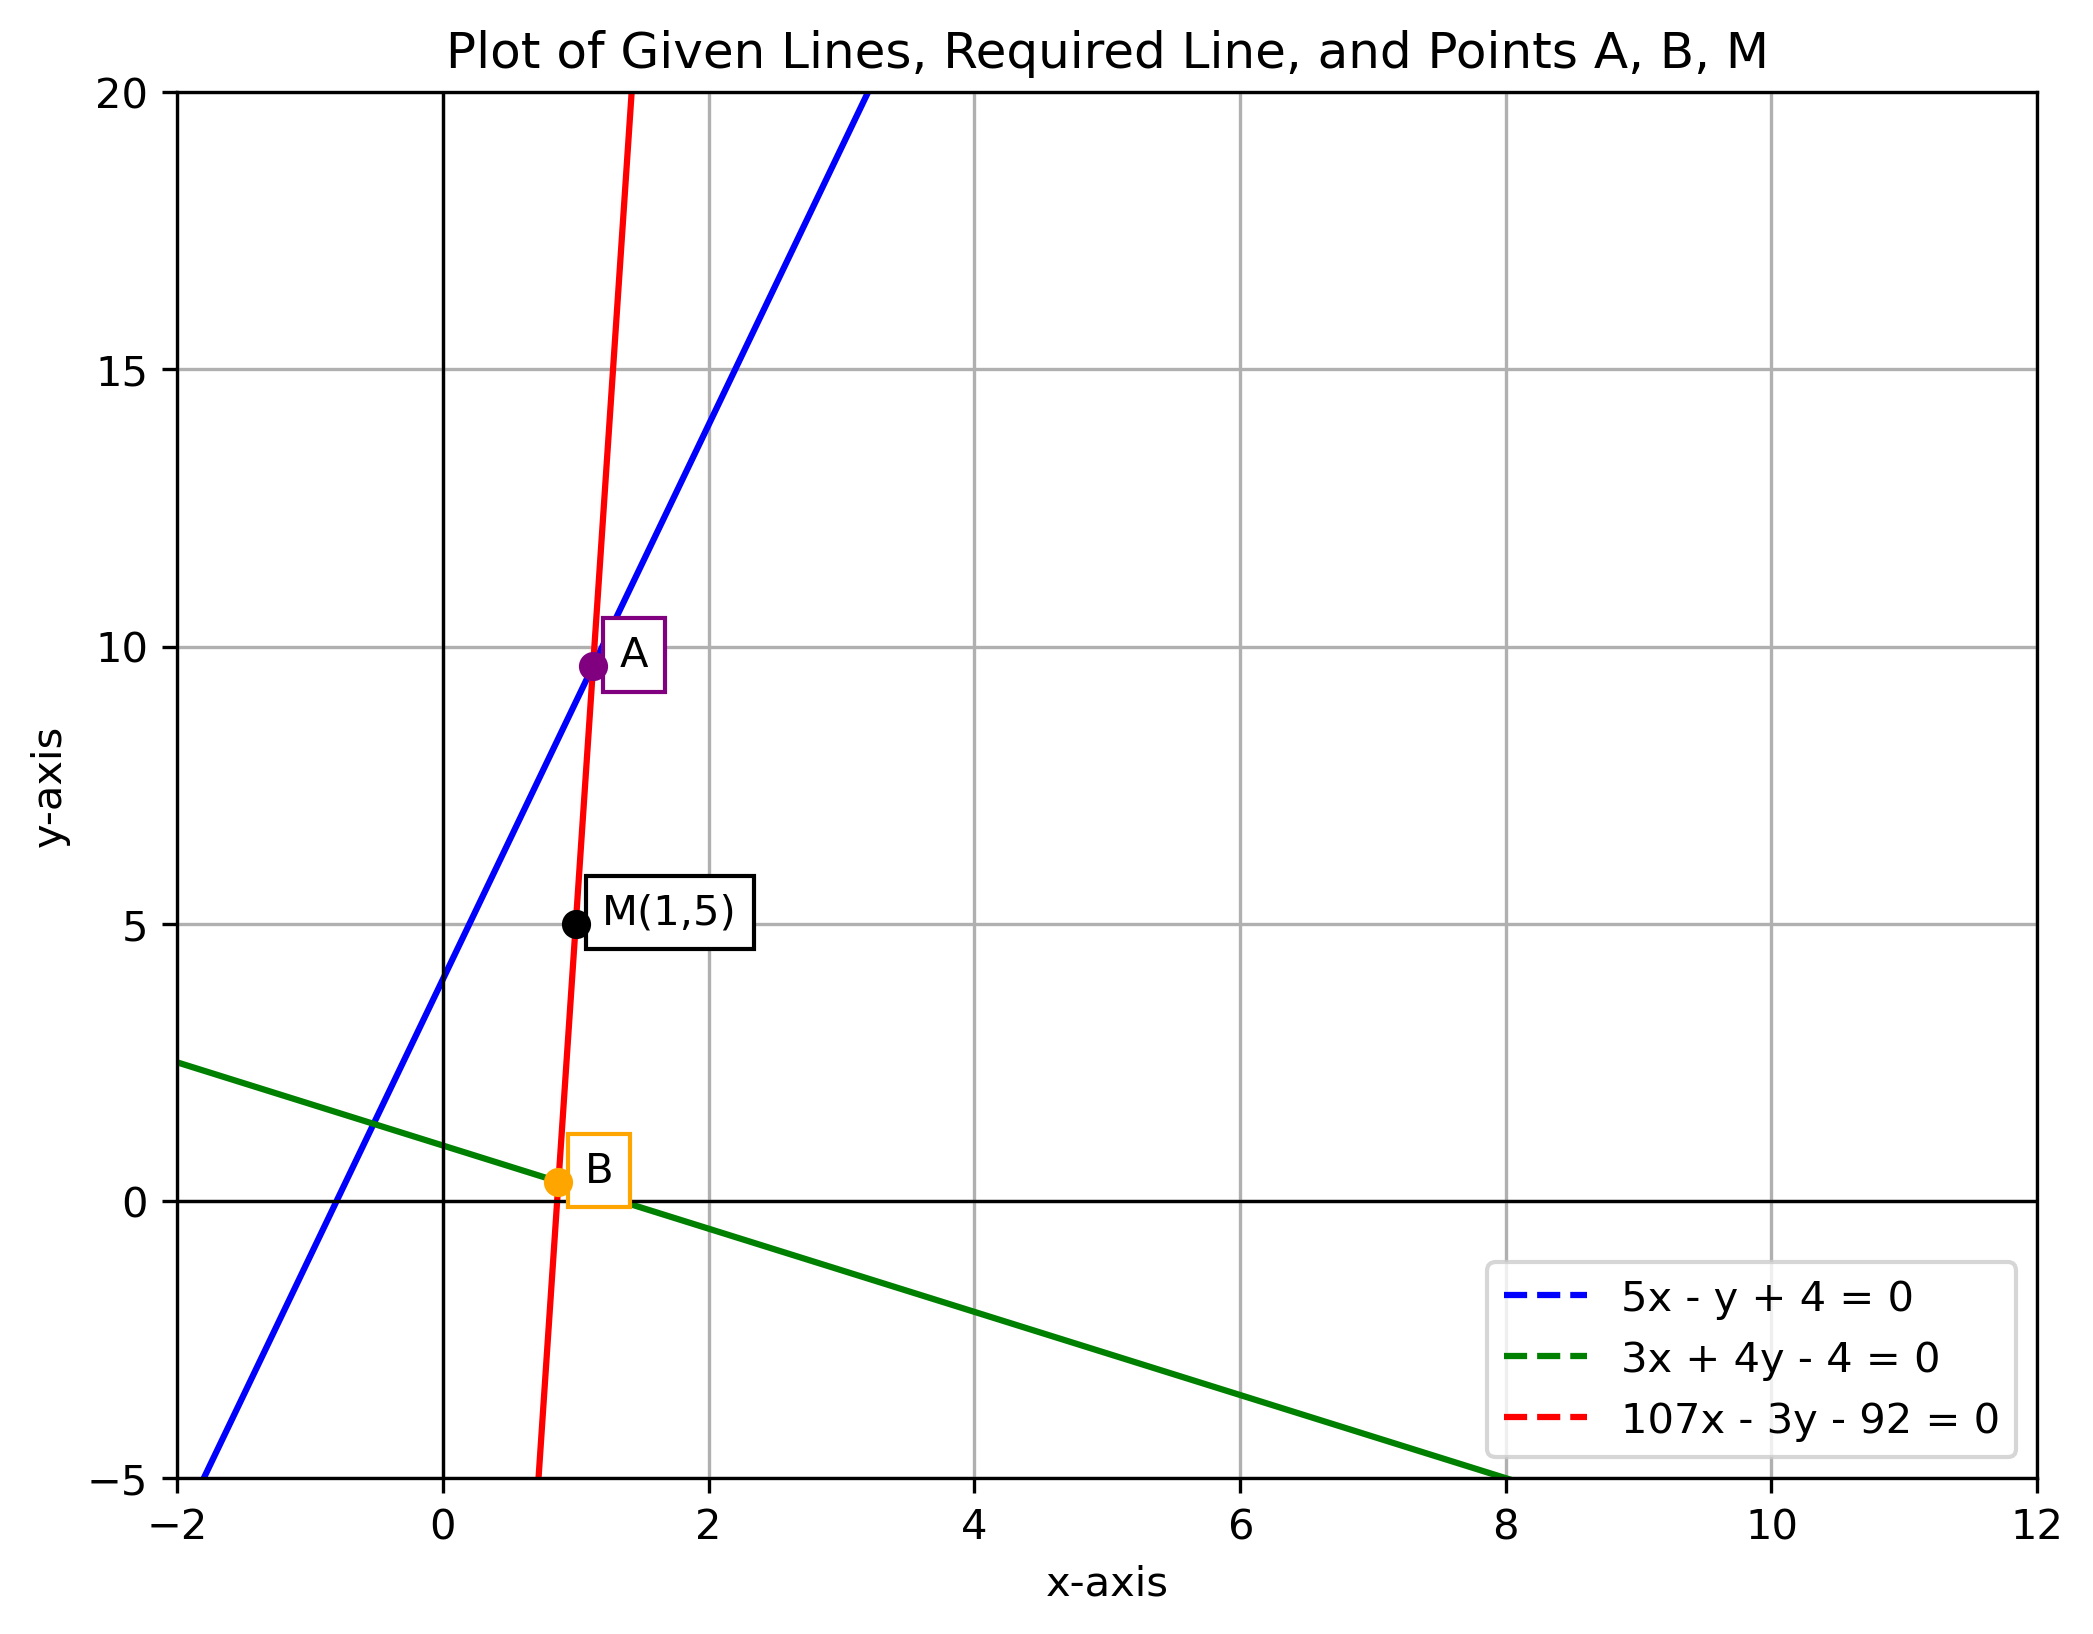
\includegraphics[width=0.8\linewidth]{figs/01.png}
    \caption{Caption}
    \label{fig:placeholder}
\end{figure}    
\end{frame}

% --------- CODE APPENDIX ---------
\section*{Appendix: Code}

% C program
\begin{frame}[fragile]{C Code: line.c}
\begin{lstlisting}[language=C]
#include <stdio.h>

int main() {
    FILE *fp;
    fp = fopen("line.dat", "w");
    if (fp == NULL) {
        printf("Error opening file!\n");
        return 1;
    }

    // Final derived equation
    fprintf(fp, "The required line equation is: 107x - 32y = 92\n");

    fclose(fp);
    printf("Output written to line.dat successfully.\n");
    return 0;
}
        \end{lstlisting}
\end{frame}

\begin{frame}[fragile]{Python: plot.py}
\begin{lstlisting}[language=Python]
import numpy as np
import matplotlib.pyplot as plt

# Define x range
x = np.linspace(-5, 15, 400)

# Define the lines
y1 = 5*x + 4           # Line 1: 5x - y + 4 = 0
y2 = (4 - 3*x) / 4     # Line 2: 3x + 4y - 4 = 0
y3 = (107*x - 92) / 3  # Line 3: 107x - 3y - 92 = 0

# Intersection points
A = (26/23, 222/23)  # ≈ (1.13, 9.65)
B = (20/23, 8/23)    # ≈ (0.87, 0.35)
M = (1, 5)           # Midpoint

# Plot solid lines
plt.figure(figsize=(8,6))
plt.plot(x, y1, color="blue")
plt.plot(x, y2, color="green")
plt.plot(x, y3, color="red")

# Create dashed proxy lines for legend
l1, = plt.plot([], [], color="blue", linestyle="--", label="5x - y + 4 = 0")
l2, = plt.plot([], [], color="green", linestyle="--", label="3x + 4y - 4 = 0")
l3, = plt.plot([], [], color="red", linestyle="--", label="107x - 3y - 92 = 0")

# Add legend box INSIDE grid
plt.legend(handles=[l1, l2, l3],
           loc="lower right", frameon=True)

# Mark the points A, B, and M (with boxes)
plt.scatter(*A, color="purple", zorder=5)
\end{lstlisting}
\end{frame} 

\begin{frame}[fragile]{Python: plot.py}
\begin{lstlisting}[language=Python]
plt.text(A[0]+0.2, A[1], "A", fontsize=10,
         bbox=dict(facecolor='white', edgecolor='purple'))

plt.scatter(*B, color="orange", zorder=5)
plt.text(B[0]+0.2, B[1], "B", fontsize=10,
         bbox=dict(facecolor='white', edgecolor='orange'))

plt.scatter(*M, color="black", zorder=5)
plt.text(M[0]+0.2, M[1], "M(1,5)", fontsize=10,
         bbox=dict(facecolor='white', edgecolor='black'))

# Axes settings
plt.axhline(0, color='black', linewidth=0.8)
plt.axvline(0, color='black', linewidth=0.8)
plt.xlim(-2, 12)
plt.ylim(-5, 20)

# Labels and grid
plt.xlabel("x-axis")
plt.ylabel("y-axis")
plt.title("Plot of Given Lines, Required Line, and Points A, B, M")
plt.grid(True)

# Save and show
plt.savefig("line_plot.png", dpi=300, bbox_inches="tight")
plt.show()

\end{lstlisting}
\end{frame} 
\end{document}
